\section{An\'alise da amostra}
\label{sec:analise}
%Fazer um estudo descritivo dos dados (gráficos e medidas). Verificar normalidade dos dados e potenciais pontos aberrantes

Nesta seção, nós apresentamos um estudo descritivo dos dados da amostra. Nesse contexto, mostramos alguns gráficos gerados por meio da linguagem R, bem como verificamos a normalidade dos dados.

\subsection{Estudo descritivo}
\label{sec:estudo}

%falar sobre os gráficos e medidas que vamos usar

\subsection{Normalidade dos dados}
\label{sec:normalidade}

%falar sobre o método de verificação da normalidade dos dados

Para demonstrar a normalidade dos dados da nossa amostra, nós usamos o teste de aderência Shapiro-Wilk~\cite{shapirowilk}. Ele testa a hipótese nula de que uma amostra foi proveniente de uma população com distribuição normal. Portanto, se o \emph{p-value} for menor do que o nível de significância escolhido, então a hipótese nula é rejeitada, ou seja, os dados não foram provenientes de uma população com distribuição normal. Por outro lado, se o \emph{p-value} for maior que o nível de significância, então a hipótese nula não é rejeitada e consequentemente, os dados são provenientes de uma população com distribuição normal. A seguir, nós formalizamos a hipótese desse teste:

\begin{equation}
	H_{0} : \text{A amostra provém de uma população Normal}
\end{equation}

\begin{equation}
	H_{1} : \text{A amostra não provém de uma população Normal}
\end{equation}

Nesse contexto, aplicando o teste Shapiro-Wilk, nós obtivemos um \emph{p-value} igual a 0,1456, que é maior que o nosso nível de significância (QUAL EH O ALPHA?). Portanto, 1 não pode ser rejeitada, o que traz evidências de que a nossa amostra provém de uma população com distribuição normal.

%% precisa falar do W também? Seria interessante olhar a tabela aqui em: http://www.portalaction.com.br/content/64-teste-de-shapiro-wilk
% nesse caso, o nosso W é 0,9546, o que é maior que 0,927 (n>=30) olhando na tabela. É mais uma evidência de normalidade

Esse teste de normalidade pode ser interpretado por um Q-Q Plot. Na Figura~\ref{fig:grafico1}, nós ilustramos a nossa análise. A reta que cruza o gráfico representa a Normal. Percebe-se que os nossos dados estão muito próximos dessa reta, com exceção somente de 4 dos 36 pontos. EXPLICAR MELHOR O GRÁFICO: EIXOS E DISCREPÂNCIAS

\begin{figure*}[t]
    \centering
    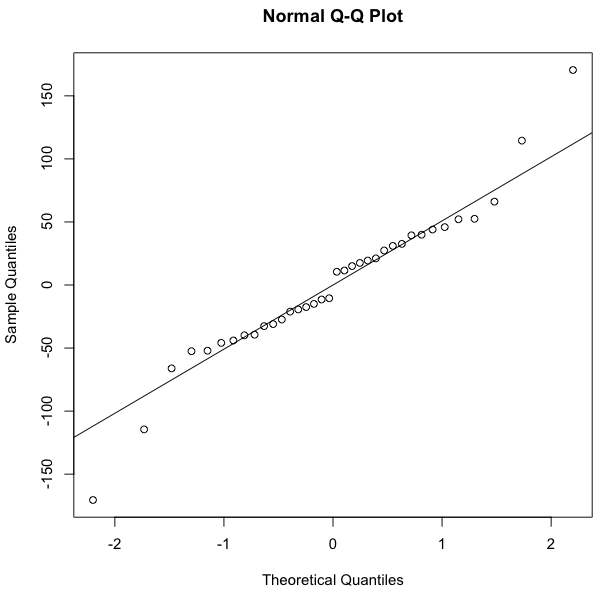
\includegraphics[width=0.4\textwidth]{images/grafico1.png}
    \caption{}
    \label{fig:grafico1}
\end{figure*}